%!BIB program=biber

\documentclass[12pt,aspectratio=169]{beamer} %类型为文章
\usepackage[UTF8]{ctex} %中文编码宏
\usepackage{multicol} %分栏控制宏
\usepackage{hyperref} %超链接宏
\usepackage{lastpage} %总计页的宏
\usepackage{color} %颜色控制宏
\usepackage{graphicx} %图片插入宏
\usepackage{subfigure} %子图插入宏
\usepackage{animate} %动画插入宏
\usepackage{multirow} %纵向合并宏
\usepackage{makecell} %表格换行宏
\usepackage{amsmath} %公式插入宏
\usepackage{unicode-math} %公式样式宏
\usepackage{gbt7714} %国标引用宏
\usepackage{url} %网页链接宏
\usepackage{doi} %doi号宏
\usepackage{svg}
\renewcommand{\vec}[1]{\boldsymbol{#1}} %设置向量样式

\usetheme{Berlin}
\usecolortheme{beaver}

\linespread{1.2} %行距
\setlength{\parskip}{0.5em} %段落间距
\setlength{\parindent}{2em} %缩进距离

\setmathfont{Cambria Math} %设置数学公式样式
%\bibliographystyle{gbt7714-numerical} %设置参考文献样式

%\logo{
\includegraphics[height=0.1\textwidth]{images/SCU_logo.pdf}}
%\setbeamertemplate{background}{
\includegraphics[height=\paperheight]{images/SCU_logo.pdf}}
\setbeamertemplate{itemize items}{$\blacksquare $}
\setbeamertemplate{caption}[numbered]


\title{工作进展回报} %设置标题
\subtitle{对傅里叶重建算法的理解}
\author{Julian OU} %设置作者
\institute[SCU]{\textit{College of Physics, Sichuan University, Chengdu 610064, China}}
\date{\today} %设置日期

\begin{document}
\maketitle %插入标题

\AtBeginSection{
    \begin{frame}
        \frametitle{目录}
        \tableofcontents[currentsection,subsectionstyle=hide]
    \end{frame}
}

\AtBeginSubsection{
    \begin{frame}
        \subsectionpage
    \end{frame}
}

\section{二维}

\subsection{单次照射}

\begin{frame}
    \frametitle{基本构想}
    \begin{figure}
        \subfigure{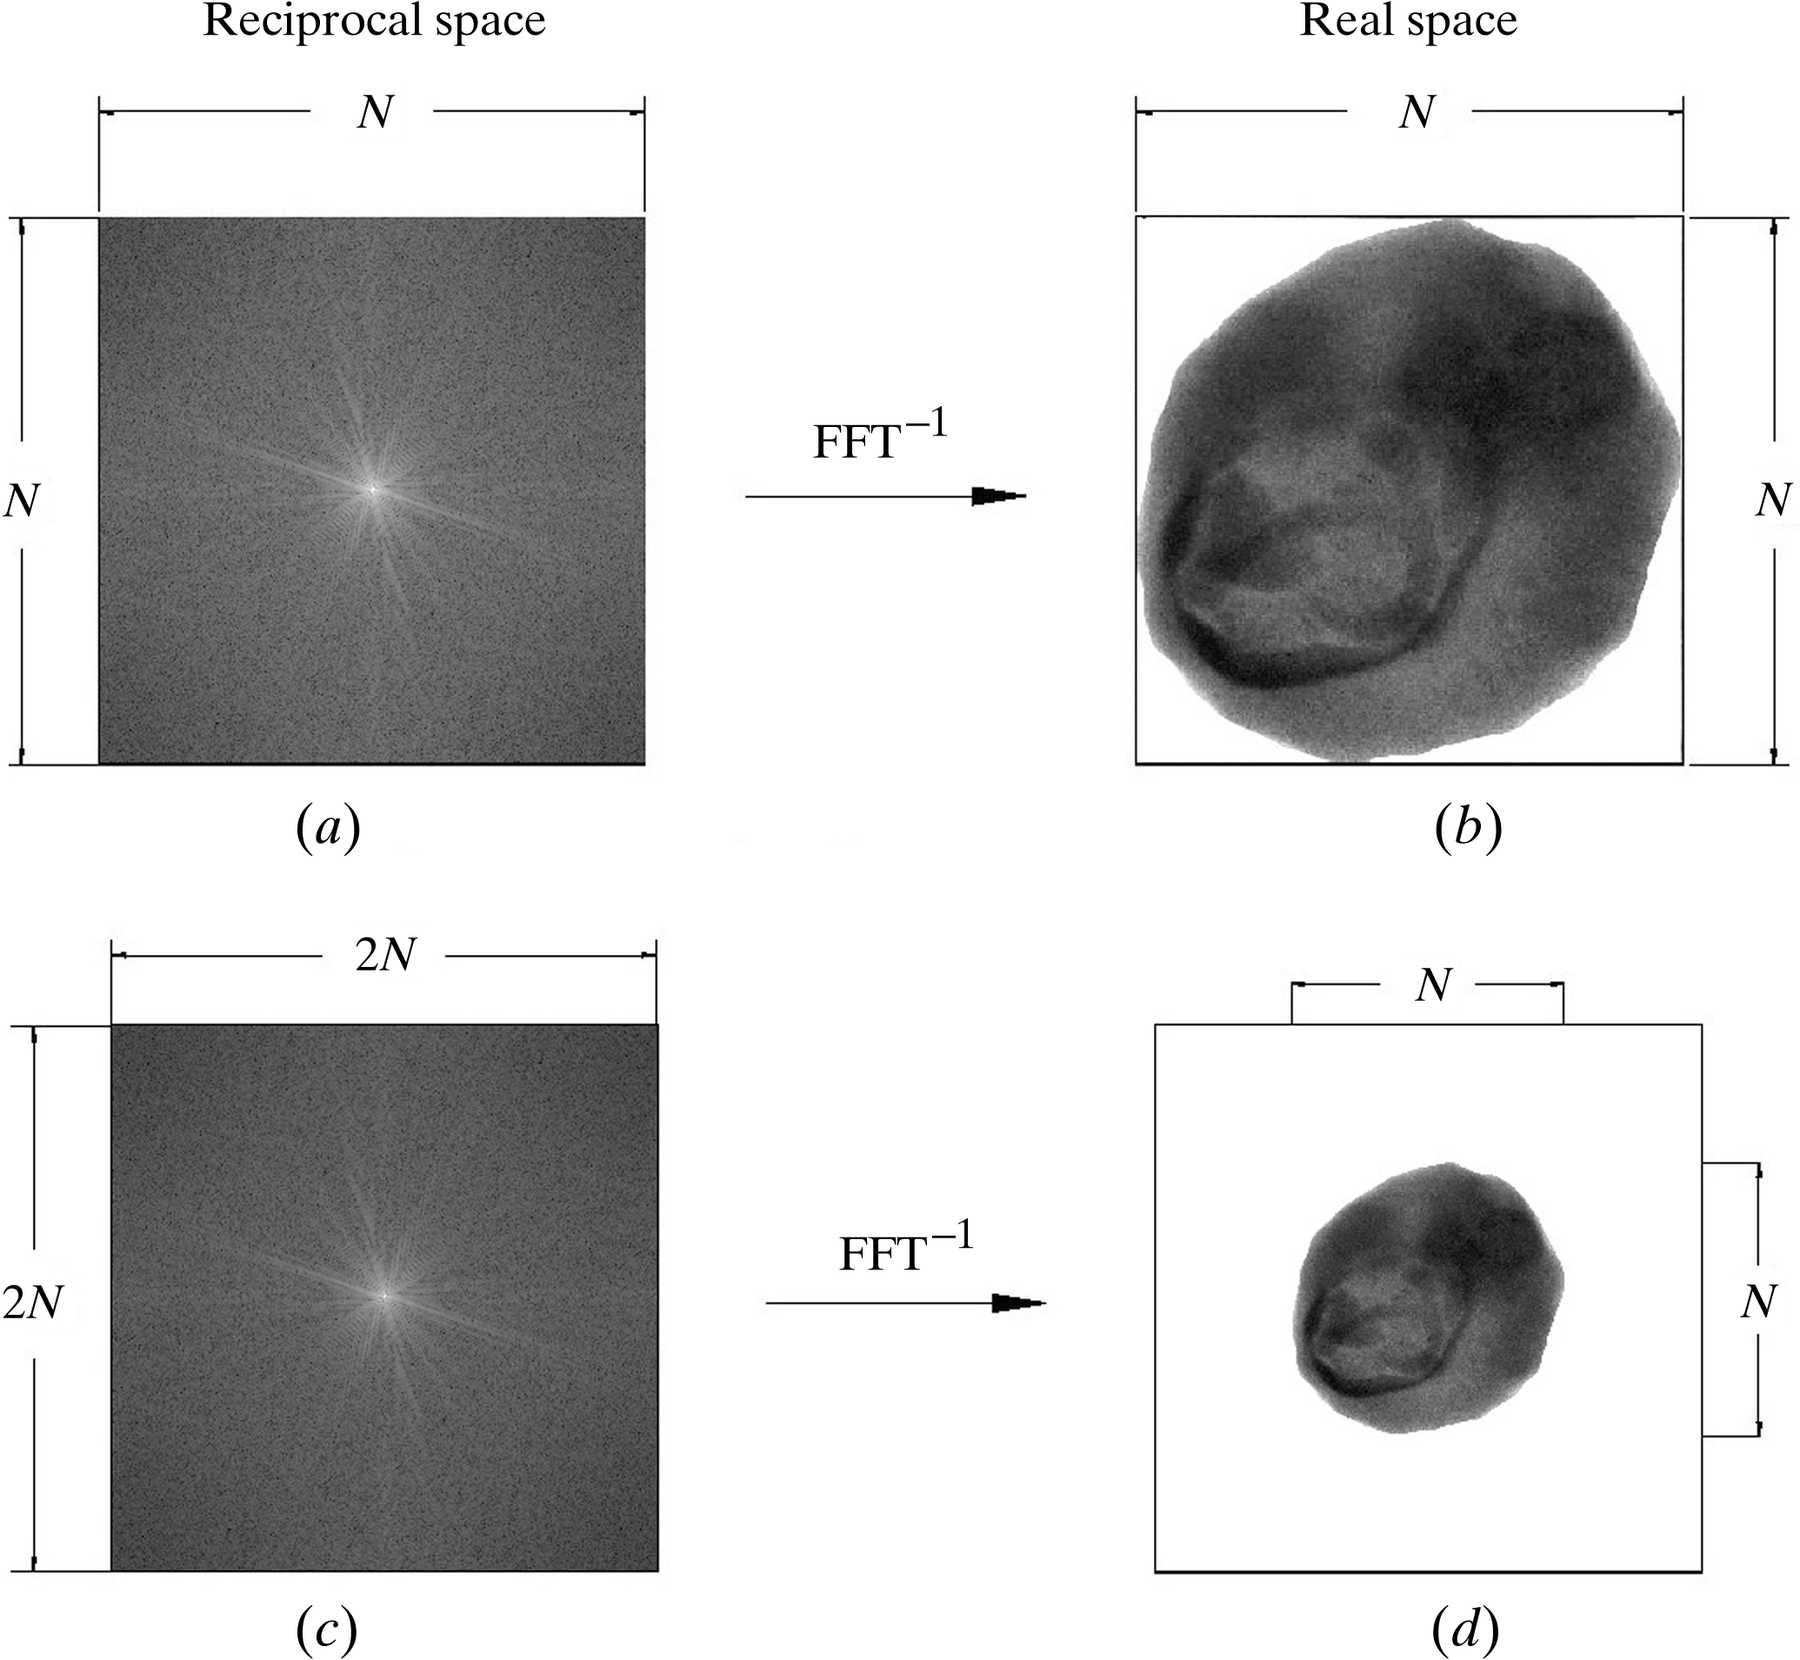
\includegraphics[height=5cm]{images/bk0084fig1mag.jpg}}
        \qquad
        \subfigure{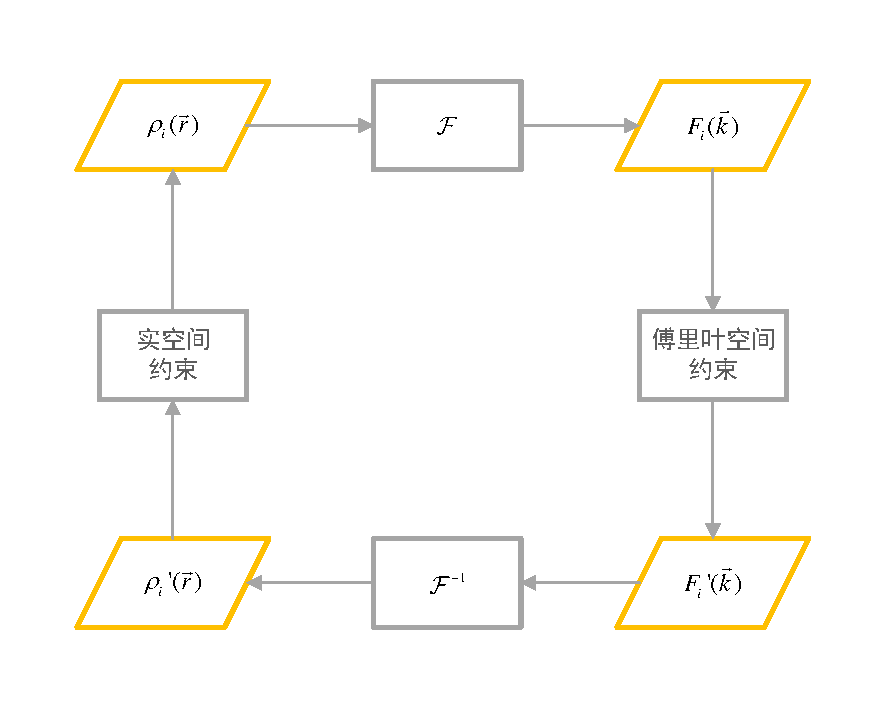
\includegraphics[height=5cm]{images/1.pdf}}
    \end{figure}
\end{frame}

\begin{frame}
    \frametitle{ER-HIO}
    \begin{figure}
        \subfigure{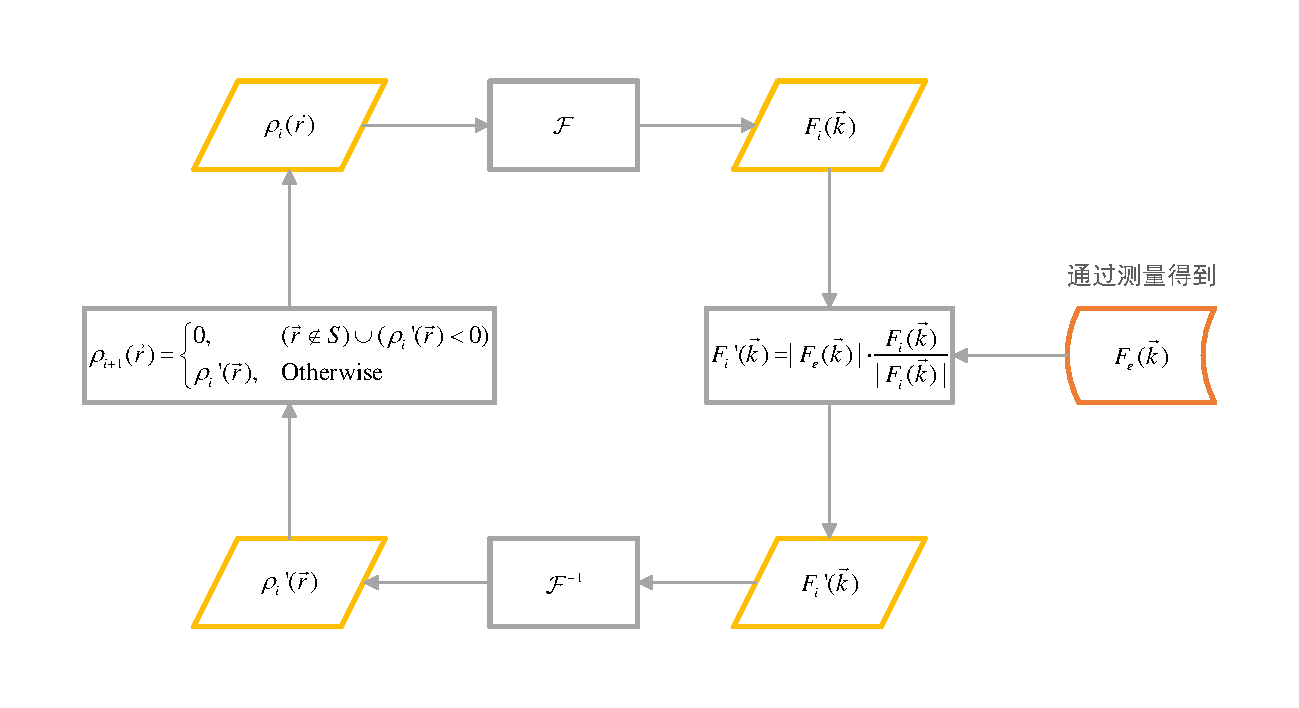
\includegraphics[height=3.6cm]{images/2.pdf}}
        \subfigure{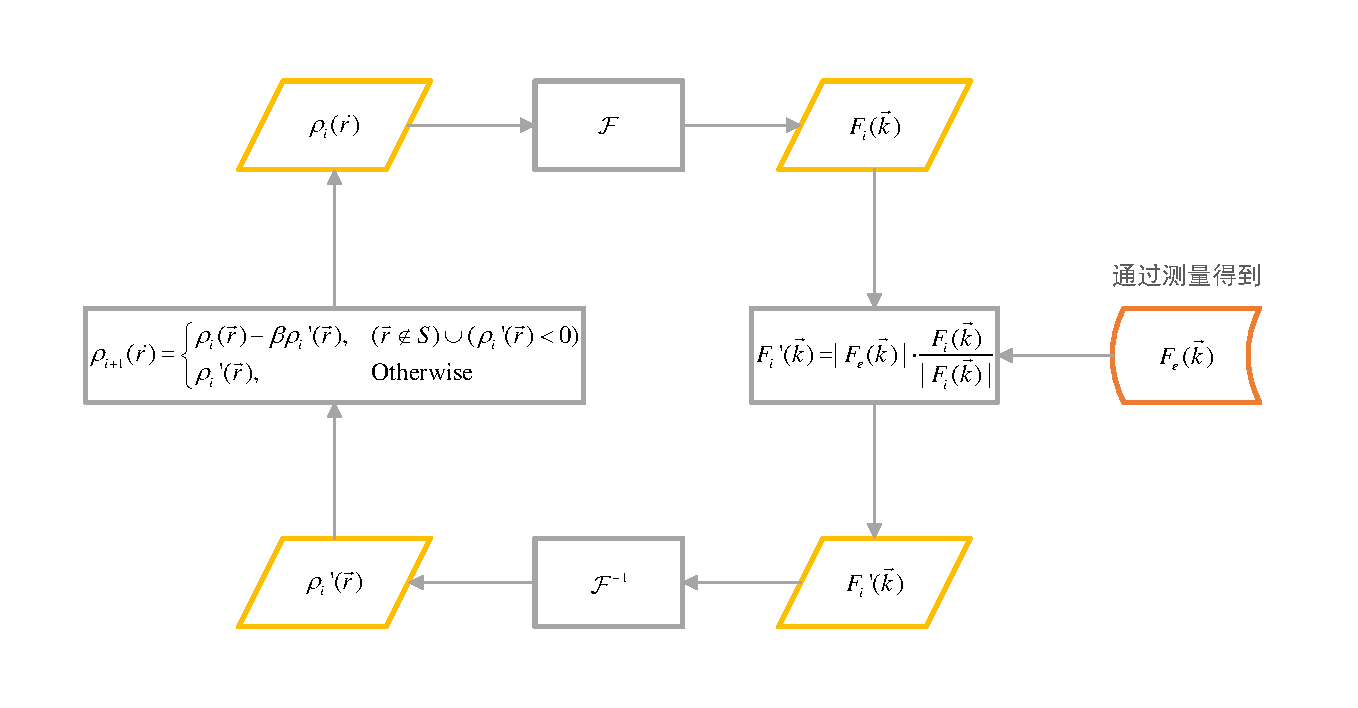
\includegraphics[height=3.6cm]{images/3.pdf}}
    \end{figure}
\end{frame}

\begin{frame}
    \frametitle{OSS}
    \begin{figure}
        \subfigure{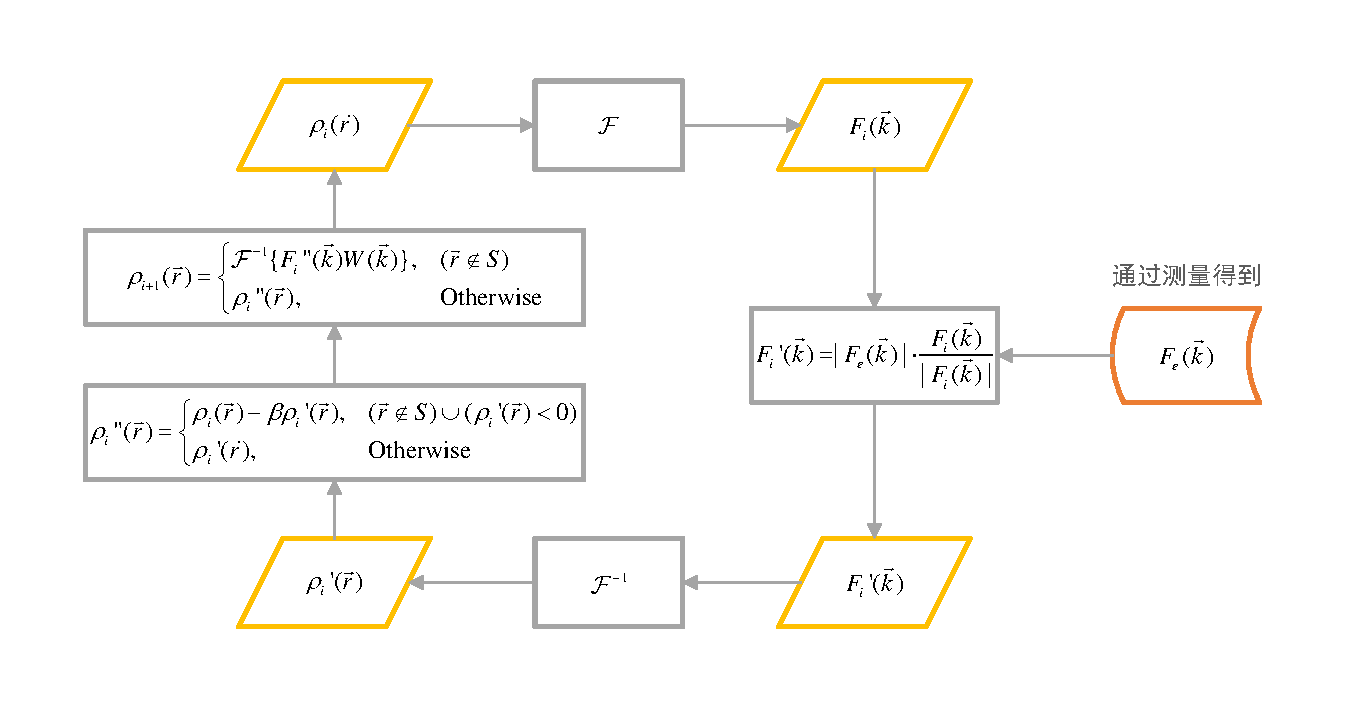
\includegraphics[height=5cm]{images/5.pdf}}
        \subfigure{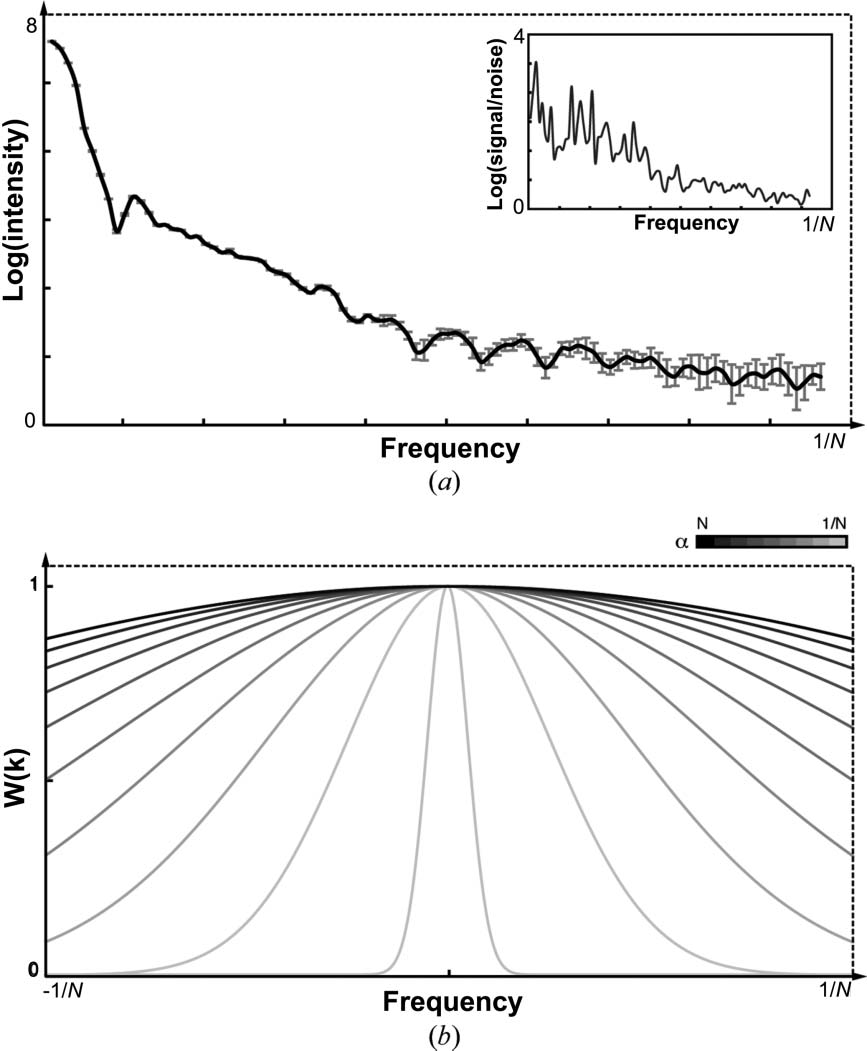
\includegraphics[height=5cm]{images/OSS_JAC_2013Oversampling smoothness-an effective algorithm.jpg}}
    \end{figure}
    

\end{frame}

\subsection{多次照射}

\end{document}